\chapter{The Atmospheric Emission Model}

Ground-based experiments have been playing and will continue to play a
prominent role in the observation of the cosmic microwave background
radiation temperature and polarisation anisotropies. As compared to
their space-borne or balloon-borne counterparts, ground-based experiments
can deploy larger primary reflectors, achieving higher angular resolution.
However, these instruments must deal with atmospheric effects.

The atmospheric radiation is almost unpolarized, therefore it does not
contribute directly to the signal acquired by instrumentation designed to
measure polarized sources, like the coherent polarimeters of the Strip
telescope. However, residual atmospheric emission inevitably increases the
optical power incident on the detectors and therefore their noise level. In
addition, temporal variations in emission, caused by variable water vapour
content, contribute low frequency correlated noise to the signal.

\section{Atmospheric Radiative Transfer}

The atmosphere can be viewed as a dielectric medium, whose effects on the
incoming electromagnetic radiation are charactherized by the complex permittivity

\begin{equation}
        \epsilon\qty(\nu) = \epsilon_r\qty(\nu) + i\epsilon_i\qty(\nu)
\end{equation}

where $\nu$ is the frequency of the incoming and radiation the real and
imaginary parts, $\epsilon_r$ and $\epsilon_i$ are linked by the
Kramers-Kronig relations

\begin{align}
        \epsilon_r\qty(s) & = \frac{1}{\pi}
        \principalvalue{\int^\infty_{-\infty}\dd{s'}
        \frac{\epsilon_i\qty(s)}{s' - s}} \label{eq:kk_relations_1} \\
        \epsilon_i\qty(s) & = -\frac{1}{\pi}
        \principalvalue{\int^\infty_{-\infty}\dd{s'}
        \frac{\epsilon_r\qty(s)}{s' - s}} \label{eq:kk_relations_2}.
\end{align}

The variable $s = \sigma + i 2\pi\nu$ is the complex frequency and $\sigma$
is the \emph{Neper frequency}.

As is shown in \autoref{fig:transmittance_teide}, contributions to the
atmospheric complex permittivity arise principally from
oxigen and water vapour molecules. Water vapour is responsible for most of
the continuum absorption in the \SIrange{400}{500}{\giga\hertz} frequency
range. The broad absorption oxigen band around \SI{60}{\giga\hertz} and the
oxigen line at \SI{119}{\giga\hertz} contribute to very strong absorption,
as the water vapour lines at \SIlist{22;183;325;380}{\giga\hertz} do. We will
show that the most problematic features of the atmospheric absorption spectrum
regarding the Q-band channels of the Strip telescope are in fact the
\SI{22}{\giga\hertz} water vapour line and the \SI{\sim 60}{\giga\hertz}
oxigen plateau.

\begin{figure}
        \centering
        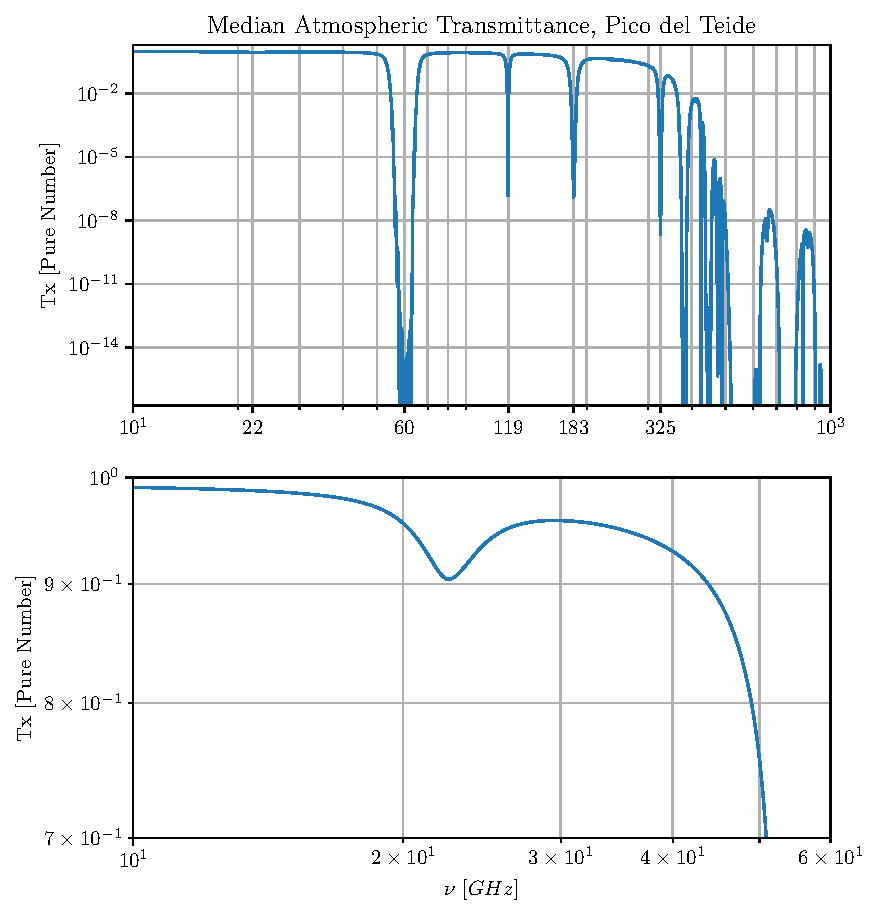
\includegraphics[width=\textwidth]{transmittance_Teide}
        \caption{Atmospheric transmittance at Pico del Teide and low
        frequencies detail. CAL software.}
        \label{fig:transmittance_teide}
\end{figure}


The real and imaginary parts of $\epsilon$ are related to the atmopshere
refractive index, $n\qty(\nu)$, and absorption coefficient, $\alpha\qty(\nu)$,

\begin{align}
        \epsilon_r\qty(\nu) & = \sqrt{n\qty(\nu)} \\
        \epsilon_i\qty(\nu) & = \frac{\lambda \alpha\qty(\nu)}{4\pi}
\end{align}

where $\lambda$ is the wavelength of the incoming radiation.

From \autoref{eq:kk_relations_1} and \autoref{eq:kk_relations_2} follows that
the refractive index and the absorption coefficient are note independent
quantities.

\subsection{Essential Quantities in Radiative Transfer Theory}

When the scale of a system greatly exceed the wavelength of propagating
radiation, we can consider radiation to travel in straight line, called
\emph{rays}. Starting from this observation we can devise a theory of
propagating rays, knwon as the \emph{radiative transfer theory}.

We consider an infinitesimal area $\dd{A}$ normal to the direction of a
specific ray and we take into account all the rays passing through $\dd{A}$
whose direction is whithin an infinitesimal solid angle $\dd{\Omega}$ of
the given ray (see \autoref{fig:rays_geometry}). The energy crossing
$\dd{A}$ in an infinitesimal time $\dd{t}$, in a frequency range $\dd{\nu}$
is

\begin{equation}
        \dd{E} \equiv
        I\qty(\vb{x},\Omega,\nu)\dd{A}dd{\Omega}\dd{\nu}\dd{t}
\end{equation}

which defines the \emph{specififc intensity}, $I\qty(\vb{x},\Omega,\nu) =
I_\nu$.

\begin{figure}
        \centering
        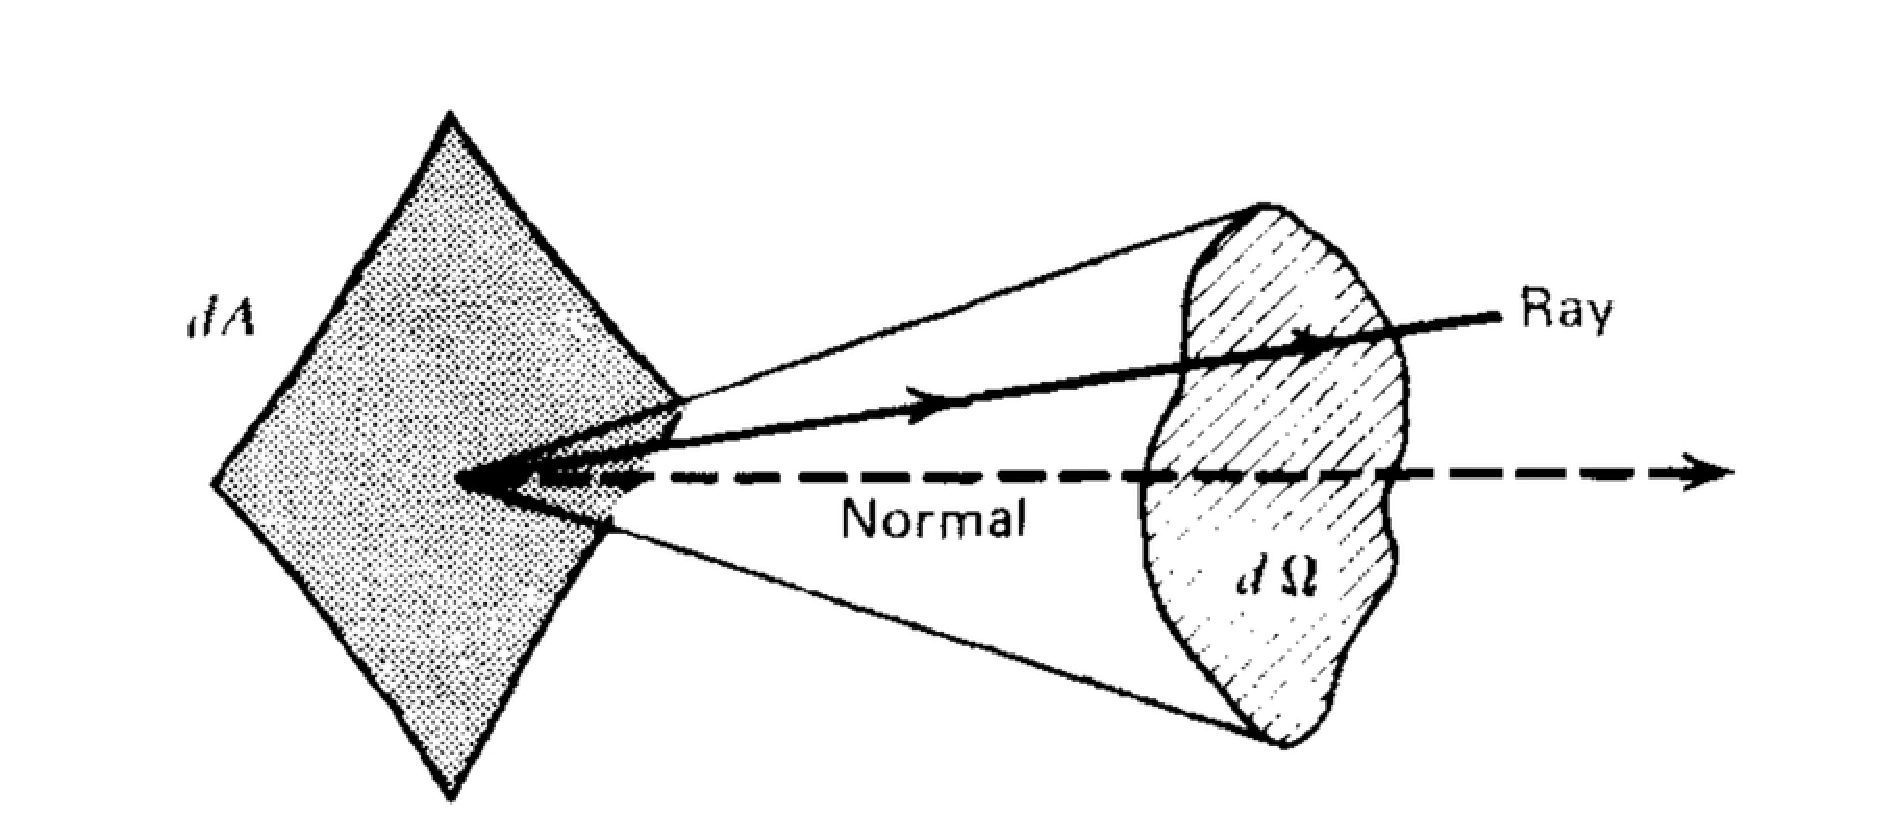
\includegraphics[width=\textwidth]{rays_geometry}
        \caption{Geometry for normally incident rays.}
        \label{fig:rays_geometry}
\end{figure}

The absorption coefficient $\alpha\qty(\nu) = \alpha_\nu$, introduced in the
previus section, represents the loss of intensity in a beam as it travels an
infinitesimal distance $\dd{r}$ in a dispersive medium. As the radiation
proceeds in the material, it runs into a random distribution of absorbers,
each presenting a cross section $\sigma_\nu$, of number density $n$. If we
assume that the mean interparticle distance is large in comparison to the
linear scale of the cross section, that is $n^{-\frac{1}{3}} \gg
\sqrt{\sigma_\nu}$, the total energy absorbed out of a beam passing
through a infinitesimal area $\dd{A}$ within a solid angle $\dd{\Omega}$ is

\begin{equation}
        \dd{E} = I_\nu \sigma_\nu n \dd{V} \dd{\Omega} \dd{\nu} \dd{t}
\end{equation}

where $\sigma_\nu n \dd{V} = \sigma_\nu n \dd{A} \dd{r}$ is the total
absorbing area presented by absorbers. The loss in energy, by definition,
can be expressed in terms of specifc brightness:

\begin{equation}
        \dd{E} = -\dd{I_\nu} \dd{A} \dd{\Omega} \dd{\nu} \dd{t}.
\end{equation}

Therefore if we combine the last two equations, we obtain

\begin{equation}
        \dv{I_\nu}{r} = -\sigma_\nu n I_\nu
        \label{eq:absorption}
\end{equation}

where $\sigma_\nu n = \alpha_\nu$. Note that absorption in
\autoref{eq:absorption} includes both \emph{true absorption} and
\emph{stimulated emission}, because both are proportional to the intensity
of the incoming radiation. Thus, $\alpha$ can be a positive or a negative
quantity.

The spontaneous emission, on the other hand, is independent of the
specific intensity of the beam. In the contest of radiative transfer theory
the quantity linked to this phenomenon is the \emph{spontaneous emission
coefficient} $j$, which is defined as the energy emitted
per unit time per unit solid angle and per unit volume:

\begin{equation}
        \dd{E} \equiv j\dd{V}\dd{\Omega}\dd{t}.
\end{equation}

A \emph{monochromatic spontaneous emission coefficient}, $j\qty(\nu) =
j_\nu$, can also be defined as

\begin{equation}
        j \equiv j_\nu \dd{\nu}.
\end{equation}

From now on we will refer to this quantity simply as the \emph{emission
coefficient}.
A beam of cross section $\dd{A}$, travelling an infinitesimal distance
$\dd{r}$, goes through a volume $\dd{V} = \dd{A} \dd{r}$. Therefore, from
the last two equations, we have

\begin{equation}
        \begin{split}
        \frac{\dd{E}}{\dd{A}\dd{\Omega}\dd{\nu}\dd{t}} & = j_\nu \dd{r} \\
        \dv{I_\nu}{r} & = j_\nu
        \label{eq:emission}
        \end{split}
\end{equation}

\subsection{The Radiative Transfer Equation}

The effects of emission and absorption can be incorporated into a sigle
equation giving the variation of specific intensity. From \autoref{eq:absorption}
and \autoref{eq:emission} we have

\begin{equation}
        \dv{I_\nu}{r} = -\alpha_\nu I_\nu + j_\nu
\end{equation}

which is known as the \emph{radiative transfer equation}. This equation
takes a particularly simple for if we realize the change of variable

\begin{equation}
        \begin{split}
                r \rightarrow \tau_\nu\qty(r) & \equiv \int^r_{r_0}
                \dd{r'}\alpha_\nu\qty(r') \\
                \dd{\tau_\nu} & = \alpha_\nu \dd{r}
        \end{split}
\end{equation}

where $\tau_\nu$ is known as the \emph{optical depth} or \emph{opacity}.
The transfer equation can now be divided by $\alpha_\nu$ and written as

\begin{equation}
        \dv{I_\nu\qty(\tau_\nu)}{\tau_\nu} = -I_\nu(\tau_\nu) +
        S_\nu\qty(\tau_\nu)
        \label{eq:radiative_transfer}
\end{equation}

where the function $S_\nu\qty(\tau_\nu)$ is known as the as the \emph{source
function} and is defined as

\begin{equation}
        S_\nu(\tau_\nu) \equiv
        \frac{j_\nu\qty(\tau_\nu)}{\alpha_\nu\qty(\tau_\nu)}.
\end{equation}

The source function and the opacity are convenient quantities in radiative
transfer theory, because they allow to reveal more clearly the intervals
along a ray that influence propagation of radiation the most.

\autoref{eq:radiative_transfer} can be now solved by regarding all
quantities as a function of the optical depth. First we multiply each side
of the equation by the positive quantity $e^{\tau_\nu}$:

\begin{equation}
        \dv{I_\nu\qty(\tau_\nu)}{\tau_\nu}e^{\tau_\nu} =
        -I_\nu\qty(\tau_\nu)e^{\tau_\nu} +
        S_\nu\qty(\tau_\nu)e^{\tau_\nu}
\end{equation}

then we integrate along a vertical path through the atmosphere:

\begin{equation}
        \begin{split}
                & \int^{\tau_{A,\nu}}_0 \dd{\tau_\nu}
                \dv{I_\nu\qty(\tau_\nu)}{\tau_\nu} e^{\tau_\nu} =
                -\int^{\tau_{A,\nu}}_0 \dd{\tau_\nu}
                I_\nu\qty(\tau_\nu) e^{\tau_\nu} +
                \int^{\tau_{A,\nu}}_0 \dd{\tau_\nu}
                S_\nu\qty(\tau_\nu) e^{\tau_\nu} \\
                & \eval{I_\nu\qty(\tau_\nu) e^\tau}^{\tau_{A,\nu}}_0
                -\int^{\tau_{A,\nu}}_0 \dd{\tau_\nu}
                I_\nu\qty(\tau_\nu) e^{\tau_\nu} = \\
                & = -\int^{\tau_{A,\nu}}_0 \dd{\tau_\nu}
                I_\nu\qty(\tau_\nu) e^{\tau_\nu} +
                \int^{\tau_{A,\nu}}_0 \dd{\tau_\nu}
                S_\nu\qty(\tau_\nu) e^{\tau_\nu} \\
                & I_\nu\qty(\tau_{A,\nu}) e^{\tau_{A,\nu}} -I_\nu\qty(0) =
                \int^{\tau_{A,\nu}}_0 \dd{\tau_\nu}
                S_\nu\qty(\tau_\nu) e^{\tau_\nu}
        \end{split}
\end{equation}

where integration by parts has been used in the right-hand side of the
equation and the quantity $\tau_{A,\nu}$ is the total opacity of the
traversed medium. If the last equation is divided by the positive factor
$e^{\tau_{A,\nu}}$ and terms are remanaged, the following equation is
obtained:

\begin{equation}
        I_\nu\qty(\tau_{A,\nu}) = I_\nu\qty(0) e^{-\tau_{A,\nu}} +
        \int^{\tau_{A,\nu}}_0 \dd{\tau_\nu}
        S_\nu\qty(\tau_\nu) e^{-\qty(\tau_{A,\nu} - \tau_\nu)}.
\end{equation}

This is known as the \emph{formal solution} of the radiative transfer
equation. The term $I_\nu\qty(0) e^{-\tau_{A,\nu}}$ represents the initial
intensity diminished by absorption and the second term in the sum stands
for the integrated source diminished by absorption.

\subsection{A Solution for Thermal Sources}

Thermal radiation is radiation emitted by matter in thermodynamic
equilibrium. When radiation is itself in thermodynamic equilibrium we
speak about \emph{black body radiation}, whose nature was already described
in \autoref{ss:cmb_bb}.

For black body radiation we have

\begin{equation}
        I_\nu \equiv B_\nu\qty(T_\text{phys})
\end{equation}

where $T_\text{phys}$ is the physical temperature of the radiation and of the
emitter and $B_\nu\qty(T_\text{phys})$ is the black body spectrum introduced
in \autoref{ss:cmb_bb},

\begin{equation}
        B_\nu\qty(T) = \frac{2h\nu^3}{c^2}
        \frac{1}{\exp(\frac{h\nu}{K_b T}) - 1}.
\end{equation}

This means that for black body radiation $I_\nu$ is an universal function
of $T$ and $\nu$, independent of the properties of the emitting body.

Kirchhoff's law states that the source function of a body in thermodynamic
equilibrium coincides with a black body spectrum

\begin{align}
        S_\nu & = B_\nu\qty(T_\text{phys}) \\
        j_\nu & = B_\nu\qty(T_\text{phys}) \alpha_\nu
\end{align}

where $T_\text{phys}$ is the physical temperature of the radiant body,
which from now on will be referred to simply as T.

The solution of the radiative transfer equation in the case of thermal
radiation is obtained from the formal solution by substitution of the
correct source function:

\begin{equation}
        I_\nu\qty(\tau_{A,\nu}) = I_\nu\qty(0) e^{-\tau_{A,\nu}} +
        \int^{\tau_{A,\nu}}_0 \dd{\tau_\nu} B_\nu\qty(T\qty(\tau_\nu))
        e^{-\qty(\tau_{A,\nu} - \tau_\nu)}.
        \label{eq:radiative_thermal}
\end{equation}

A further approximation can be made to simplify this result.
The exponential term in the Planck law can be expanded as

\begin{equation}
       \exp(\frac{h\nu}{K_b T}) = 1 + \frac{h\nu}{K_b T} + \order{\nu^2}.
\end{equation}

Therefore, for $\frac{h \nu}{K_b T}$, we obtain the \emph{Rayleigh-Jeans
approximation law}:

\begin{equation}
        B_\nu\qty(T) \approx \frac{2\nu^2}{c^2} K_b T.
\end{equation}

This relation is commonly used in astrophysics to characterize the
brightness of a radiation at a certain frequency. For any value value of
$I_\nu$ a corresponding \emph{brightness temperature} temperature can be
defined as

\begin{equation}
        I_\nu \equiv B_\nu\qty(T_b)
\end{equation}

or assuming that the Rayleigh-Jeans approximation is valid,

\begin{equation}
        T_b \equiv = \frac{c^2}{2\nu^2k} I_\nu.
\end{equation}

So, \autoref{eq:radiative_thermal} can be rewritten as

\begin{equation}
        T_b = T_b\qty(0) e^{-\tau_{A,\nu}} +
        \int^{\tau_{A,\nu}}_0 \dd{\tau_\nu} T\qty(\tau_\nu)
        e^{-\qty(\tau_{A,\nu} - \tau_\nu)}.
\end{equation}

The solution of this equation in the case of constant temperature along the
optical path, $T\qty(\tau_\nu) = T = \text{const.}$ is

\begin{equation}
        T_b = T_b\qty(0) e^{-\tau_{A,\nu}} + T\qty(1 -
        e^{-\tau_{A,\nu}}).
\end{equation}

If the opacity is large, the brightness temperature of the radiation
approaches the temperature of the medium.

particle velocities within it corresponds to the \emph{Maxwell-Boltzmann}
distribution,

\begin{equation}
        p\qty(v) = \qty(\frac{m_*}{2\pi K_b T})^{3/2}
        \exp(-\frac{m_* v^2}{2 K_b T})
\end{equation}

where $m_*$ is a reference mass for particles in the atmosphere.
This means that in principle we can split the atmosphere in an arbitrary
number of vertical layers, assuming the thermodynamic temperature is
constant within each one.  The radiative transfer equation can then be
written down and solved for every layer and the solutions connected. This
constitutes a simplified view of the numerical approach we have adopted in
the context of this thesis to obtain estimates for atmospheric brightness
temperatures.

\section{Atmospheric Spatial Structures}
